% -*-latex-*-

%% IMPORTANT: The official thesis specifications are available at:
%%            http://libraries.mit.edu/archives/thesis-specs/
%%
%%            Please verify your thesis' formatting and copyright
%%            assignment before submission.  If you notice any
%%            discrepancies between these templates and the
%%            MIT Libraries' specs, please let us know
%%            by e-mailing thesis@mit.edu

%% The documentclass options along with the pagestyle can be used to generate
%% a technical report, a draft copy, or a regular thesis.  You may need to
%% re-specify the pagestyle after you \include  cover.tex.  For more
%% information, see the first few lines of mitthesis.cls.

%\documentclass[12pt,vi,twoside]{mitthesis}
%%
%%  If you want your thesis copyright to you instead of MIT, use the
%%  ``vi'' option, as above.
%%
%\documentclass[12pt,twoside,leftblank]{mitthesis}
%%
%% If you want blank pages before new chapters to be labelled ``This
%% Page Intentionally Left Blank'', use the ``leftblank'' option, as
%% above.

\documentclass[12pt,oneside]{mitthesis}
\usepackage{lgrind}
\usepackage{amsmath,amssymb}
%% These have been added at the request of the MIT Libraries, because
%% some PDF conversions mess up the ligatures.  -LB, 1/22/2014
\usepackage{cmap}
\usepackage[T1]{fontenc}
\usepackage{indentfirst}
\usepackage{mathrsfs}

\usepackage[colorlinks=true,bookmarks=true]{hyperref}
  \usepackage{bookmark}
  \hypersetup{breaklinks=true}

\usepackage{geometry}
\geometry{
    a4paper,
    left=1.5in,
    right=1.0in,
    top=1.0in,
    bottom=1.0in
}

\usepackage{fancyhdr}
\fancypagestyle{plain}{
    \fancyhf{} % clear all header and footer fields
    \fancyhead[R]{\thepage} % page number in top right
    \renewcommand{\headrulewidth}{0pt}
    \renewcommand{\footrulewidth}{0pt}
}

%%todo packages
\usepackage[colorinlistoftodos]{todonotes}

%% Addtional packages
\usepackage{lipsum}

%% This bit allows you to either specify only the files which you wish to
%% process, or `all' to process all files which you \include.
%% Krishna Sethuraman (1990).

%\typein [\files]{Enter file names to process, (chap1,chap2 ...), or `all' to process all files:}
%\def\all{all}
%\ifx\files\all \typeout{Including all files.} \else \typeout{Including only \files.} \includeonly{\files} \fi

\newcommand{\mysignrule}[0]{
    \rule{\linewidth}{0.5pt}\newline
}

%-------------------------------------------
\begin{document}

\hypersetup{pageanchor=false}
\pagenumbering{roman}
\title{The Onset of Color Transparency in Quasielastic ${}^{12}C(e,e'p)$ Scattering}

\makeatletter
\author{John Matter} \let\Author\@author
\newcommand{\hometown}{Moreno Valley, CA}

\prevdegrees{B.S., University of Califoria, Davis, 2012}
\department{Department of Physics}
\degree{Doctor of Philosophy}
\degreemonth{June}
\degreeyear{2020} \let\Year\@degreeyear
\thesisdate{June 1, 2020}
\makeatother

\supervisor{Nilanga Liyanage}{Professor}
\chairman{Kent Paschke}{Professor}

\makeatletter
\def\maketitle{\begin{titlepage}
\doublespacing
\vspace{0.0in}
\large
{\LARGE\bf \@title \par}
\@author \\
\hometown
\par
\@prevdegrees
\par
A Dissertation Presented to the Graduate Faculty \\
of the University of Virginia in Candidacy for the Degree of \\
\@degree
\par
\@department \\
University of Virginia \\
\@degreemonth, \@degreeyear \\
\vspace{1.0in}

\begin{flushright}
\begin{minipage}{0.45\linewidth}
\mysignrule{}
\mysignrule{}
\mysignrule{}
\mysignrule{}
\end{minipage}
\end{flushright}

\end{titlepage}}
\makeatother
\maketitle

% Copyright page
\pagenumbering{roman}
\pagestyle{plain}
\newpage
\vspace*{\fill}
\noindent \textcopyright Copyright by \Author {} \Year \\
All Rights Reserved

\cleardoublepage

% Abstract page
\vspace{0.8in}
\pdfbookmark[0]{Abstract}{Abstract}
\section*{\center Abstract}
% -*-latex-*-
%
% $Log: abstract.tex,v $
% Revision 1.1  93/05/14  14:56:25  starflt
% Initial revision
%
% Revision 1.1  90/05/04  10:41:01  lwvanels
% Initial revision

%% The text of your abstract and nothing else (other than comments) goes here.
%% It will be single-spaced and the rest of the text that is supposed to go on
%% the abstract page will be generated by the abstractpage environment. This
%% file should be \input (not \include 'd) from cover.tex.

\noindent
This is the abstract section. You should replace this with your own abstract.

%%%%%%%%%%%%%%%%%%%%%%%%%%%%%%%%%%%%%%%%%%%%%%%%%%%%%%%%%%%%%%%%%%%%%%
% -*-latex-*-


\cleardoublepage

% Acknowledgemnt page
\pdfbookmark[0]{Acknowledgments}{Acknowledgments}
\section*{Acknowledgments}
This is the acknowledgement section.


\hypersetup{pageanchor=true}

\hypersetup{linkcolor=black}
\pagestyle{plain}
% -*-latex-*-

%% This file simply contains the commands that actually generate the table of
%% contents and lists of figures and tables.  You can omit any or all of
%% these files by simply taking out the appropriate command.  For more
%% information on these files, see appendix C.3.3 of the LaTeX manual.

\tableofcontents
\newpage
\listoffigures
\newpage
\listoftables
\cleardoublepage

%%%%%%%%%%%%%%%%%%%%%%%%%%%%%%%%%%%%%%%%%%%%%%%%%%%%%%%%%%%%%%%%%%%%%%
% -*-latex-*-

\hypersetup{linkcolor=red}

\pagenumbering{arabic}
\chapter{Introduction}
\label{ch1}
Condensed matter physics is primarily centered around the exploration of phases and phase transitions. This domain experienced a significant advancement in the mid-20th century, when Landau and Ginzburg formulated a comprehensive theory of phases and transitions \cite{Landau:1937obd,Ginzburg:1950sr}. According to Landau's theory, unique phases are characterized by the distinct symmetries of their ground states. The transitional process from one phase to another is unable to occur without an accompanying break in these symmetries.
An illuminating example of this principle is observed in the transition between phases of water. When water solidifies into ice, its continuous translational symmetry is disrupted, leading to the establishment of a discrete translational symmetry. This change transpires as atoms align to form a crystalline structure. The phase transition from water to ice necessitates a disruption of the initial symmetry. Conversely, the transition between the states of water and vapor maintains a consistent translational symmetry. This indicates that these two states can interconvert without a phase transition, thereby showing them equivalent. As illustrated in the phase diagram of water, depicted in Figure \ref{fig:water}, a smooth transformation from water to vapor is achievable when one surpasses the critical point. In conjunction with symmetry breaking, Landau and Ginzburg introduced order parameters which have quantized value to distingush distinct phases.

\begin{figure}[h]
    \centering
    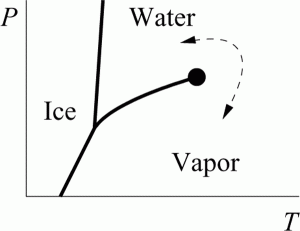
\includegraphics[width =0.5\textwidth]{images/water.png}
    \caption{The phase diagram of water. The solid boundaries between the phases indicate phase transitions. When we go beyond the critical point, we can transform between water and vapor without going through phases transition. }
    \label{fig:water}
\end{figure}

\begin{figure}[h]
    \centering
    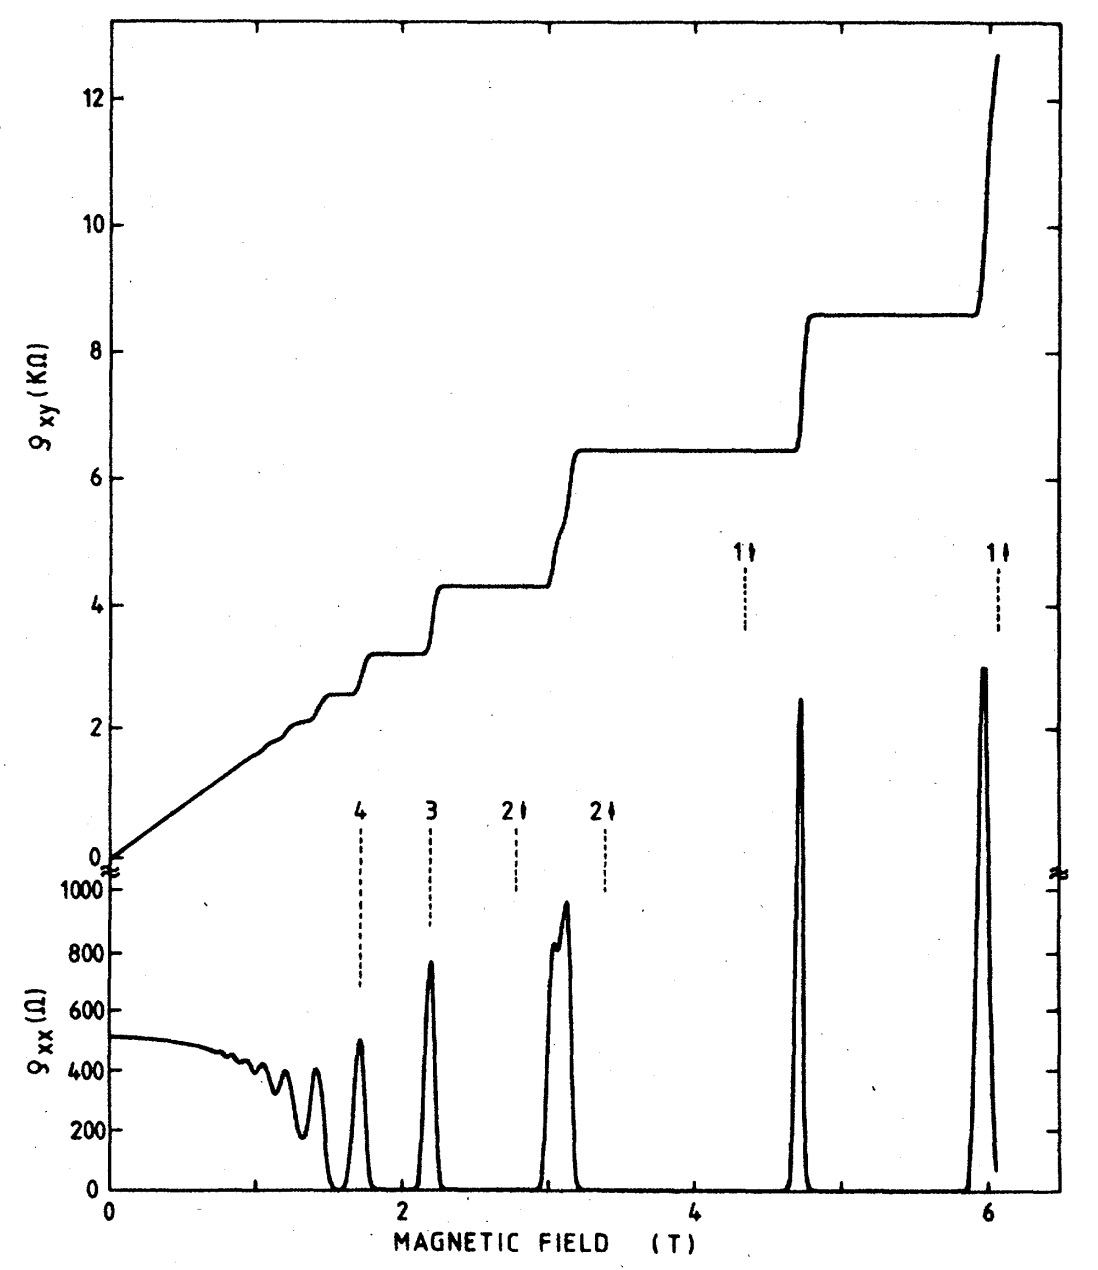
\includegraphics[width =0.5\textwidth]{images/qhe.jpg}
    \caption{Experimental curves for Hall conductance.\cite{von1986quantized}As the magnetic field increases, the quantized plateau of Hall conductance becomes apparent.}
    \label{fig:qhe}
\end{figure}

Landau's paradigm was accepted as the universal framework capable of describing all phases of matter and continuous phase transitions for a long time. This longstanding consensus began to evolve in the 1980s, however, following the discovery of the Quantum Hall Effect\cite{von1986quantized}. This significant breakthrough revealed that certain quantum phases did not conform to the traditional tenets of Landau's paradigm. In the Quantum Hall Effect, the Hall conductance becomes quantized at low temperatures. As the magnetic field is incrementally adjusted, the Hall conductance transitions between quantized Hall plateaus. Intriguingly, this phase transition occurs without any associated symmetry breaking, even as the magnetic field is simply being tuned. This marked the dawn of a thrilling new area of study which is called topological phases that expands upon the classic Landau symmetry-breaking paradigm to accommodate phases that transcend its traditional boundaries.

There are two kinds of topological phases: topological ordered phase and symmetry protected topological(SPT) phases. The Quantum Hall Effect serves as a typical example of topological ordered phases. Meanwhile, the recent discovery of topological insulators and superconductors in the 21st century has revealed a diverse range of SPT phases  with the presence of symmetries.

The principle of adiabatic continuity is employed to differentiate between topological phases. Two gapped quantum phases are considered topologically distinct if their Hamiltonians cannot be smoothly interconnected without closing a gap.  In the meantime, a trivial phase must be established as a reference point for studying non-trivial topological phases, which exhibit exotic collective behaviors.
 For a system with $n$ atoms, if the total Hilbert space is a direct product of each local Hilbert space, represented as $$\mathscr H = \bigotimes_{n\in \mathbb Z}  \mathscr H^{loc}_n$$
 , then the ground state is also in a product state, which we refer to as a trivial system. Any system that can be smoothly transitioned to this product state is deemed equivalent to the trivial phase.


Topological phases, unlike trivial product states, cannot be smoothly deformed and are noted for their exotic collective behaviors. Topological ordered phases, for instance, are long-range entangled phases that can exist independently of any symmetries. They are capable of hosting fractional or non-Abelian quasiparticles with corresponding fractional or non-Abelian statistics and are characterized by ground state degeneracy which depends on the topology of the underlying geometry. The family of fractional quantum Hall states, which host anyons, belong to this category. Another type of topological order, the toric code, exhibits a four-fold degeneracy on a torus geometry, while presenting a single ground state on a cylinder. This demonstrates the direct relationship between spatial topology and topological order.

On the other hand, symmetry protected topological (SPT) phases are short-range entangled phases protected by symmetries. When the symmetries protecting the topological phases are disrupted, SPT phases can be smoothly transformed into trivial states. This is why they are called "symmetry protected". Contrary to topological order, SPT phases do not host any quasiparticles in the bulk, but their bulk Hamiltonian is characterized by bulk topological invariants. Both topological order and SPT phases host non-trivial edge states.

The topological properties of topological order are robust against any form of perturbation. In contrast, for SPT phases, the topological properties are only robust to perturbations that preserve symmetries. A comparison of topological order and SPT phases is summarized in Table \ref{tab:comparison}.



Beyond this fundamental classification, topological phases are differentiated based on the specific symmetries that protect them and the dimensions of the system in question. Our exploration will concentrate on SPT phases and the alignment of actual materials with the characterization of topological phases. The complex interplay between symmetry, topology, defects, and atomic hopping significantly augments the diversity of topological phases of matter.

* topological: global property
* math and physcs correspondence



\begin{table}[]
\renewcommand{\arraystretch}{1.5}
\label{tab:comparison}
\begin{tabular}{|l|l|l|}
\hline
             & Topological Order & SPT Phases \\\hline
Symmetries   & No symmetry required    &  Must protected by symmetries \\\hline
Edge states  &   Yes   &   Yes  \\\hline
Ground States & Degenerated & Unique \\\hline
Exotic Bulk & Can host anyons even be & \\
Quasiparticle &  fractional or non-Abealian & No \\\hline
Entanglement &  Long range        &  Short range   \\\hline
Perturbation  &  Robust against any perturbation & Perturbations have to\\ 
 & &preserve symmetries\\
\hline
\end{tabular}
\caption{Comparison of Topological Order and SPT Phases}

\end{table}

\section{Classification of gapped topological phases.}
As previously introduced, Symmetry Protected Topological (SPT) phases do not fit within the Landau-Ginzburg symmetry-breaking theory. Consequently, when dealing with two different phases sharing the same symmetry, no local order parameter can be used to distinguish them. Reflecting on the Quantum Hall Effect, where quantized Hall conductivity represents different topological phases, it becomes intuitive to associate a set of quantized invariants with topological phases, effectively characterizing the universality class. One way to determine if two phases with same symmetries are topologically equivalent to each other is by comparing the values of these invariants. 
These quantized invariants, referred to as topological invariants, function in a manner analogous to principle quantum numbers in atoms, where they denote different states.

For a free fermion system in a lattice, we can use a tight-binding Hamiltonian to describe it. 
\begin{align}
\hat{H}=\sum_{r,r'}\psi^\dagger(r)H(r,r')\psi(r')
\end{align}
where $\psi(r)$ is fermion annihilation operator with N degrees of freedom. $\hat{H}$ is the total Hamiltonian and $H(r,r')$ is a $N\times N$ matrix. A superconductor system can be described by Bogoliubov-de Gennes (BdG) Hamiltonian with Nambu spinors in a similar format. Under the lattice translation symmetry, we can apply Fourier transformation and get the Hamiltonian in momentum space: 
\begin{align}
\label{eq:HK}
    H = \sum_{k\in BZ}\psi^\dagger(k) H(k)\psi(k)
\end{align}
where $H(k) = \sum_re^{-ik\cdot r}H(r)$ and $k$ represents the momentum in Brillouin zone. 


(later link to K theory group homology)


*  topological features in physics phenomenon/ physicsal meaning of topological invariants----QHE as example
\subsection{Ten-fold classification}

The ten-fold classification categorize topological phases under time reversal symmetry ($T$), particle hole symmetry ($C$) and chiral symmetry ($S$). The act on the system and apply constrains to its Hamiltonian.
\begin{align}
\label{eq:TCS}
    TH(k)T^{-1} = H(-k)\\
    CH(k)C^{-1} = -H(-k)\\
    SH(k)S^{-1} = -H(k)
\end{align}
where $T^{2} = \pm 1, C^2 = \pm 1, S^2 = 1$. Both time reversal symmetry (TRS) and particle-hole symmetry (PHS) are antiunitary symmetries. In the case of spin-1/2 fermions, the square of the TRS yields $-1$, while in systems devoid of spin-orbit coupling, the square of the TRS produces $+1$. The PHS manifests in superconducting systems and, when acting on the Nambu space, results in $C^2 = +1$. Under the influence of spin symmetry in a superconducting system, it can square to $-1$. Both chiral symmetry and PHS are antisymmetry which leads to the negative sign in front of the Hamiltonian. Chiral symmetry is a combination of TRS and PHS.  In the presence of TRS and PHS, chiral symmetry is guaranteed; however, it can also exist even when TRS and PHS are both absent.


Altland and Zirnbauer, considering the existence and the squaring of the previous three symmetries, classified quantum phases into ten distinct categories, as shown in the first column of Table\ref{tab:10fold} \cite{altland1997nonstandard}. In the subsequent column, '0' indicates the absence of the respective symmetries, '+' and '-' denote the squaring of symmetries, and '1' signifies the existence of Chiral symmetry, since S is always squared to 1. The respective topological classifications can be appropriately filled in once we elaborate on K-theory and Bott periodicity.


\begin{table}[h]
\label{tab:10fold}
\begin{tabular}{|c|ccc|cccccccc|}
\hline
AZ class\textbackslash d & T & C & S & 0 & 1 & 2 & 3 & 4 & 5 & 6 & 7 \\ \hline
A                        & 0 & 0 & 0 & $\mathbb{Z}$  & 0   &$\mathbb{Z}$  &0   &$\mathbb{Z}$  &0   &$\mathbb{Z}$   &0   \\
AIII                     & 0 & 0 & 1 &   &$\mathbb{Z}$   &0   &$\mathbb{Z}$   &0   &$\mathbb{Z}$   &0   &$\mathbb{Z}$   \\ \hline
AI                       & + & 0 & 0 &$\mathbb{Z}$   &0   &0   &0   &2$\mathbb{Z}$   &0   &$\mathbb{Z}_2$   &$\mathbb{Z}_2$   \\
BDI                      & + & + & 1 &$\mathbb{Z}_2$   &$\mathbb{Z}$   &0   &0   &0   &2$\mathbb{Z}$   &0   &$\mathbb{Z}_2$   \\
D                        & 0 & + & 0 &$\mathbb{Z}_2$   &$\mathbb{Z}_2$   &$\mathbb{Z}$   &0   &0   &0   &2$\mathbb{Z}$   &0   \\
DIII                     & - & + & 1 &0   &$\mathbb{Z}_2$   &$\mathbb{Z}_2$   &$\mathbb{Z}$   &0   &0   &0   &2$\mathbb{Z}$   \\
AII                      & - & 0 & 0 &2$\mathbb{Z}$   &0   &$\mathbb{Z}_2$   &$\mathbb{Z}_2$   &$\mathbb{Z}$   &0   &0   &0   \\
CII                      & - & - & 1 &0   &2$\mathbb{Z}$   &0   &$\mathbb{Z}_2$   &$\mathbb{Z}_2$   &$\mathbb{Z}$   &0   &0   \\
C                        & 0 & - & 0 &0   &0   &2$\mathbb{Z}$   &0   &$\mathbb{Z}_2$   &$\mathbb{Z}_2$   &$\mathbb{Z}$   & 0  \\
CI                       & + & - & 1 &0   &0   &0   &2$\mathbb{Z}$   &0   &$\mathbb{Z}_2$   &$\mathbb{Z}_2$   &$\mathbb{Z}$  \\
\hline
\end{tabular}
\caption{Periodic table for Ten-fold classification of topological insulators and superconductors in various dimensions. A value of 0 under the symmetry column represents the lack of local symmetries, while the 0 under dimension column signifies the absence of a topological phase within a specific symmetry class and spatial dimension.}
\end{table}


\subsection{K-theory framework}
There are several equivalent methods for determining the classification of phases, including the use of homotopy groups of classifying space, K-theory, and Clifford algebra.  Mathematically, those approaches are equally potent in classifying topological phases and elucidating corresponding physical phenomena.
Here we will introduce the K-theory framework, which was initially proposed by Kitaev to assign topological invariants to various quantum phases. By leveraging the Bott periodicity\cite{atiyah1964clifford} result derived from K-theory, we can develop a periodic table which classifies SPT phases periodically in dimension with assorted symmetries, thereby laying the groundwork for classification problems.

Mathematically, topological K-theory associate a ring $K(X)$ and a given topological space $X$, thus offering an invariant capable of differentiating phasses of mater. It was developed in the 1960s by Hirzebruch and Atiyah\cite{atiyah1967K}. K-theory is geometrically expressed using vector bundles and can be expanded into a cohomology theory with Bott periodicity. Essentially, K-theory is the classification of vector bundles. However, it doesn't rely on homotopy equivalence, but instead uses stable equivalence. This approach allows the addition, or direct sum, of trivial bundles. The concept of stable equivalence is such that two vector bundles, $E_1$ and $E_2$, are stably equivalent if they become isomorphic upon the addition of trivial bundles, denoted as 
\begin{equation}
    E_1\oplus \epsilon^n \approx E_2\oplus \epsilon^m
\end{equation} for some $m$, $n$.

As we have previously discussed, the classification of topological phases can initially be viewed as the homotopy classification of maps from the base space (Brillouin zone) to the classifying space of the Hamiltonian, defined as:
\begin{equation}
    h:\mathbf{k}\rightarrow H(\mathbf{k})
\end{equation}
Two Hamiltonian belong to the same topological phases if the maps are smoothly connected to each other. In SPT phases, symmetries imposes constrain to the classifying space. By extending homotopy equivalence to stable equivalence, we can expand the equivalent Hamiltonian or classifying spaces by adding extra trivial bands. Although we generally focus on energy levels near the band gap and aim to reduce the Hamiltonian size when examining their characteristics, stable equivalence enables us to identify a collection of Hamiltonians of various sizes that can be deformed into one another by the addition of trivial bands.
\begin{equation}
    H_1\sim H_2
\end{equation}This group of Hamiltonians defines the family of topologically equivalent phases.

To illustrate the concept of finding the classifying space, let's consider the example of the Integer Quantum Hall Effect. This phenomenon, which occurs in two dimensions, does not necessitate any specific symmetry for its topological protection. By using a linear approximation near the $\Gamma$ point in the Brillouin Zone, we can derive a Dirac Hamiltonian:

\begin{equation}
H(\mathbf{k}) = k_x\sigma_1+k_y\sigma_2+m\sigma_3
\end{equation}

When we incorporate the trivial bands into our analysis without the symmetry constraint, the Hamiltonians can be described by:

\begin{equation}
C_0 = U(n+m)/(U(n)\times U(m))
\end{equation}

In this equation, the unitary matrices $U(n+m)$ are used to diagonalize the Hamiltonian, while $U(n)$ and $U(m)$ represent unitary rotations of the conduction bands and valence bands, respectively. The mapping from the Brillouin Zone to the classifying space would therefore be:
\begin{equation}
P:\mathbb{T}^2\rightarrow U(n+m)/(U(n)\times U(m))
\end{equation}
Finally, the homotopy that demonstrates the different topological phases is given by $\pi_0(C_0) = \mathbb{Z}$. Similar to IQHE, we can find the complex and real classifying space for Hamiltonians under different symmetries. Their corresponding classification are summrized in table \ref{tab:bottC} and table \ref{tab:bottR}.

One important application of K-theory is the Bott periodicity. It was proven by Raoul Bott through Morse theory and shows different isomorphism structure for complex and real classifying space\cite{bott1956application}. When applied to Symmetry Protected Topological (SPT) phases within the Altland-Zirnbauer (AZ) class, the K group periodicity can be summarized as follows:
\begin{align}
K_{\mathbb{C}}(s;d) = \pi_0(C_{s-d}) [s=0,1 (mod 2)]\\
K_{\mathbb{R}}(s;d) = \pi_0(R_{s-d}) [s=0,1,...,7 (mod 8)]
\end{align}
where, $K_{\mathbb{C}/\mathbb{R}}(s;d)$ represents the K groups for complex and real classifying spaces of $s$ AZ class in $d$ dimensions. Leveraging the results from tables \ref{tab:bottC} and \ref{tab:bottR}, we can fill in the "Tenfold Way" classification table, \ref{tab:10fold}. This illustrates periodicity across both dimensions and AZ classes.

In the Ten-fold table \ref{tab:10fold}, the renowned topological insulator in both two and three dimensions is classified as class AII. It is protected by time reversal symmetry and exhibits gapless modes along its edges while remaining insulating in the bulk. The $\mathbb{Z}_2$ classification reveals that insulators in this class can be categorized as either topological or trivial. When the invariant can assume values from the entire integer group, we employ $\mathbb{Z}$ to represent distinct topological phases corresponding to different values. The integer quantum Hall effect, on the other hand, falls under class A with integer invariants. Researchers have also discovered other Symmetry Protected Topological (SPT) phases that conform to this classification.


\begin{table}[h]
\renewcommand{\arraystretch}{1.5}
\caption{Bott periodicity in complex K-theory}
\label{tab:bottC}
\begin{tabular}{l|l|l}
\hline
q mod 2 & Classifying space $C_q$  & $\pi_0(C_q)$ \\\hline
0       & $(U(k+m)/(U(k)\times U(m)))\times \mathbb{Z}$ & $\mathbb{Z}$   \\
1       & $U(n)$   & 0                        \\\hline
\end{tabular}
\end{table}

\begin{table}[]
\renewcommand{\arraystretch}{1.5}
\caption{Bott periodicity in Real K-theory}
\label{tab:bottR}
\begin{tabular}{l|l|l}
\hline
q mod 8 & Classifying space $R_q$  & $\pi_0(R_q)$ \\\hline
0       & $(O(k+m)/(O(k)\times O(m)))\times \mathbb{Z}$ & $\mathbb{Z}$   \\
1       & $O(n)$   & $\mathbb{Z}_2$     \\
2       & $O(2n)/U(n)$   & $\mathbb{Z}_2$     \\
3       & $U(2n)/Sp(n)$   & 0   \\
4       & $(Sp(k+m)/Sp(k)\times Sp(m)\times\mathbb{Z}$   & $\mathbb{Z}$     \\
5       & $Sp(n)$   & 0     \\
6       & $Sp(n)/U(n)$   & 0     \\
1       & $U(n)/O(n)$   & 0    \\\hline

\end{tabular}
\end{table}


\subsection{Topological invariant}
\label{sec:invariant}
From the ten fold classification table, we observe an important patten while decending the dimension the topological invariant goes $\mathbb{Z}\rightarrow\mathbb{Z}_2\rightarrow\mathbb{Z}_2$. The exact number of topological invariants are used to determine different phases as well as showing different physical response. It is crucial that we are able to calculate them. Here we summarize the definition of topological invariants using bulk bloch wave function\cite{chiu2016classification}. 

For the Hamiltonian in momentum space in equation \ref{eq:HK}, we can diagonalize it to get the $i$-th eigenfunction
\begin{equation}
    H(\mathbf{k})|u^a(\mathbf{k})\rangle = E^a(\mathbf{k})|u^a(\mathbf{k})\rangle
\end{equation}
there is a energy gap seperating the $m$ valence bands and $n$ conduction bands where $N=m+n$.

In even dimension d or non-chiral classes, the integer invariant $\mathbb{Z}$ is characterized using Chern number.
\begin{equation}
\label{eq:chern}
    Ch_n = \frac{1}{n!}(\frac{i}{2\pi})^n\int_{BZ^d}Tr(F^n)
\end{equation}
where $Ch_n$ is the $n$-th Chern number and $n=d/2$. The Berry curvature can be calculated by the filled bands.
\begin{equation}
    F = dA+A^2
\end{equation}
where $A$ is the non-Abelian Berry connection:
\begin{equation}
    A^{ab} = \langle u^a(\mathbf{k})|d|u^b(\mathbf{k})\rangle = \langle u^a(\mathbf{k})|\frac{d}{d\mathbf{k}}|u^b(\mathbf{k})\rangle d\mathbf{k}
\end{equation}
Topologically, the Chern number identifies the obstruction of the mapping from the Brillouin space to the Bloch function. As the dimension increases, the Chern number may diminish. This is exemplified in 2D class A systems such as the Chern insulator\cite{haldane1988model}. Here, the integer topological invariant Chern number corresponds to the quantized Hall conductance observed in Quantum Anomalous Hall Effect experiments. The experimental discovery of the Chern insulator in thin films of Cr-doped (Bi,Sb)$_2$Te$3$, InAs/GaSb, and Hg${1-y}$Mn$_y$Te quantum wells\cite{chang2013experimental, wang2014quantum,liu2008quantum} is a case in point.

For odd dimension $d=2n+1$, a winding number can be defined when the system has chiral symmetry $S$. The chiral symmetry applies a constrain to the free fermion Hamiltonian showing in equation \ref{eq:TCS}. It is covenient to introduce a "flattened Hamiltonian" which has the same Hilbert space as the original Hamiltonian with energy levels squashed to $\pm 1$ through projecting the energy bands to valence bands
\begin{align}
    Q(\mathbf{k})=1-2P(\mathbf{k})\\
    P(\mathbf{k}) = \sum|u(\mathbf{k})\rangle\langle u(\mathbf{k})|
\end{align}
where $P(\mathbf{k})$ is the projector.
With chiral symmetry, it is always possbible to transform the Bloch Hamiltonian into a block off diagonal form
\begin{equation}
    Q(\mathbf{k})= \begin{pmatrix}
0 & q(\mathbf{k}) \\
q\dagger(\mathbf{k}) & 0 
\end{pmatrix}
\end{equation}
where $q(\mathbf{k})$ is unitary. The integer winding number is given by:
\begin{equation}
    \nu_{2n+1}[q]=\frac{(-1)^nn!}{(2n+1)!}(\frac{i}{2\pi})^{n+1}\int_{BZ}Tr[(q^{-1}dq)^{(2n+1)}].
\end{equation}
Three-dimensional class DIII topological superconductors are characterized by a winding number in their Bogoliubov-de Gennes (BdG) Hamiltonian. The physical implication of this three-dimensional winding number is the surfacing of Majorana cones, which is responsible for the quantization of thermal Hall conductivity. A compelling example of this is evident in the B-phase of superfluid 3-He\cite{volovik2003universe,schnyder2008classification,qi2009time}. While it has been established that this phase forms a topological superfluid, the realization of topological superconductivity has yet to be demonstrated conclusively in any known material or system.

The $\mathbb{Z}_2$ invariants, which are the first and second decendent of Chern number and winding number while lowering the dimension, can be represented by the Fu-Kane invariant and Chern-Simons term.

The Chern-Simons invariant can be defined in odd $d = 2n+1$ dimension. 
\begin{equation}
    \mathrm{CS}_{2 n+1}[\mathcal{A}]:=\int_{\mathrm{BZ}^d} \mathcal{Q}_{2 n+1}(\mathcal{A})
\end{equation}
it integrates the Chern-Simons term $\mathcal{Q}$ over the Brillium zoon
\begin{align}
& \mathcal{Q}_{2 n+1}(\mathcal{A}):=\frac{1}{n !}\left(\frac{i}{2 \pi}\right)^{n+1} \int_0^1 d t \operatorname{Tr}\left(\mathcal{A} \mathcal{F}_t^n\right) \\
& \mathcal{F}_t=t d \mathcal{A}+t^2 \mathcal{A}^2=t \mathcal{F}+\left(t^2-t\right) \mathcal{A}^2
\end{align}
This invariant is not quatized in general but it can be quantized in the presence of symmetries. With antiunitary symmetry like time reversal symmetry, the  Chern-Simons invariant will be quantized into half-integers
\begin{equation}
\mathrm{CS}_{2 n-1}=\int_{\mathrm{BZ}^d} \mathcal{Q}_{2 n-1} \in \frac{1}{2} \mathbb{Z}
\end{equation}
thus the $\mathbb{Z}_2$ invariant can be defined:
\begin{align}
    &\mathbb{Z}_2 = 0, \text{when } \mathrm{CS}_{2n-1}\in \mathbb{Z} + \frac{1}{2} \\
    &\mathbb{Z}_2 = 1, \text{when } \mathrm{CS}_{2n-1}\in \mathbb{Z}.
\end{align}
In the one-dimensional Kitaev chain of class D\cite{kitaev2001unpaired}, the trivial and topological Chern-Simons invariants reflect the absence or presence of Majorana zero modes at the chain's boundary, respectively. The Kitaev chain serves as a crucial experimental platform for exploring Majorana physics, encompassing fusion rules and non-Abelian exchange statistics. Moreover, it holds significant potential for applications in fault-tolerant quantum computing. Recent experimental advancements have provided compelling evidence of Majorana zero modes in platforms such as InSb/NbTiN\cite{gul2018ballistic} and InAs/Al\cite{deng2016majorana}.

The well-known three-dimensional topological insulator, which belongs to class AII due to the existence of time reversal symmetry, is characterized by its $\mathbb{Z}_2$ Chern-Simons invariant. Non-trivial phases of this class possess conducting surface states, the stability of which is safeguarded by time reversal symmetry. The Bi${1-x}$Sb$_x$ alloy, the first known 3D topological insulator, was initially predicted by Fu and Kane in 2006\cite{fu2007topological}. This prediction was subsequently confirmed by angle-resolved photoemission spectroscopy (ARPES) experiments, which observed the surface states in 2008\cite{hsieh2008topological}.The quantized Chern-Simons invariant is equivalent to the Pfaffian invariant of the gluing matrix $w^{\alpha\beta}(\mathbf{K}) = \left\langle u^\alpha(-\mathbf{k}) \mid T u^\beta(\mathbf{k})\right\rangle$. This equivalence is apparent between a time-reversal invariant momentum (TRIM) point and its time-reversal partner\cite{fu2007topological, wang2010equivalent, ando2013topological}. The Pfaffian invariant is given by the following equation:
\begin{equation}
W=\prod_{\mathrm{K}} \frac{\operatorname{Pf}[w(\mathbf{K})]}{\sqrt{\operatorname{det}[w(\mathbf{K})]}}.
\end{equation}


The $\mathbb{Z}_2$ Fu-Kane invariant is defined as integration of berry curvature over the half Brillium zone and the integration of Chern-Simons term over the boundary of the half Brillium zone. The other half of the Brillium zone is connected by the symmetry operator. Similar to the Chern-Simons invariant, the constraint from the symmetry forces the Fu-Kane invariant taking a $\mathbb{Z}_2 = \{0, 1\}$ value.
\begin{equation}
\mathrm{FK}_n=\frac{1}{n !}\left(\frac{i}{2 \pi}\right)^n \int_{\mathrm{BZ}_{1 / 2}^d} \operatorname{Tr}\left(\mathcal{F}^n\right)-\oint_{\partial \mathrm{BZ}_{1 / 2}^d} \mathcal{Q}_{2 n-1},
\end{equation}
The topological insulator in two-dimension which is also a class AII topological phases, is described by Fu-Kane $\mathbb{Z}_2$ invariant\cite{fu2006time}.


%\section{Classification of gapless topological phases.}
%\subsection{different type of gapless mode}
%* what is Weyl/Dirac semimetal
%\subsection{Classification of gapless topological phases with 2 fold megenetic symmetry(march meeting pre)}

\section{Charge density wave(CDW)}
\subsection{CDW and spontaneous symmetry breaking}
In condensed matter systems, many phase transitions can be understood as spontaneous symmetry breaking, a idea first proposed by Landau. Spontaneous symmetry breaking occurs when the ground state of a system exhibits only a subset of the symmetry present in its underlying Hamiltonian, as illustrated in the fig \ref{fig:symmetry_breaking}. This phenomenon is a fundamental concept in condensed matter physics and is closely related to the concept of order parameters and critical phenomena. By studying the behavior of systems near the critical point of a phase transition, researchers can gain insights into the underlying mechanisms that drive the spontaneous symmetry breaking and the resulting changes in the physical properties of the system. The study of spontaneous symmetry breaking has played a key role in advancing our understanding of a wide range of materials, including magnets, superconductors, and liquid crystals, and has important implications for many technological applications.

\begin{figure}[h]
    \centering
    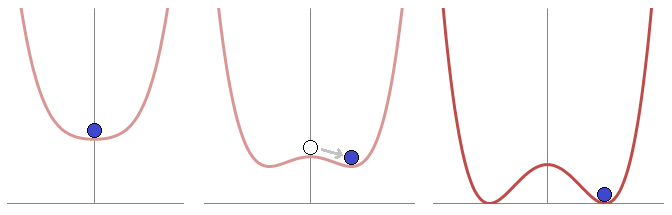
\includegraphics[width =\textwidth]{images/Spontaneous_symmetry_breaking_(explanatory_diagram).png}
    \caption{Illustration of Spontaneous symmetry breaking. The temperature decreases from left to right. The underlying Hamiltonian(represented by the red line) is always symmetric. However, as we lower the temperature, the system undergoes a phase transition, leading to a change in the ground state of the system. At high temperatures, the ground state (represented by a ball) is symmetric, but as the temperature decreases, the ground state of the system changes to another state with lower symmetry.  }
    \label{fig:symmetry_breaking}
\end{figure}

Charge density waves (CDWs) are one example of a physical phenomenon that arises from spontaneous symmetry breaking. In a CDW, the electronic charge density of a material undergoes a periodic modulation, breaking the translation symmetry of the crystal lattice. This results in a new, lower-energy ground state that is not invariant under the original symmetry. 

The CDW state is characterized by a spontaneous symmetry breaking phenomenon. As a result, it cannot be continuously connected to the high-temperature symmetric state, and a phase transition is required to enter the CDW phase. This is because spontaneous symmetry breaking cannot occur without undergoing a phase transition, as the symmetry must be broken to reach the lower-energy state. The Peierls transition \cite{Peierls1956QuantumTO} is an example of a phase transition that is often associated with the formation of CDWs.

\subsection{CDW in one dimension: Peierls transition}
\label{ch:cdw1d}

 Consider a metal in which the ions are arranged in a periodic lattice structure at their equilibrium positions. Fig\ref{fig:Peierls}(a) shows a one-dimensional linear chain with one atom per unit cell and a lattice constant $a_0$. The tight-binding model with nearest neighbor hopping $t$ gives a band dispersion of
\begin{align}
E(k) = -2t \cos{ka_0}
\end{align}
for a half-filled band with the Fermi surface located at $k_F = \frac{\pi}{2a_0}$, connected by a wave vector $q=2k_F$.However, Peierls demonstrated that this system is unstable at low temperatures, and a lattice distortion, which is a consequence of electronic disturbance and moves every other atom closer to each other, can open up a gap near the Fermi energy. This distortion changes the lattice periodicity to $2a_0$ and the unit cell is now enlarged to contain two atoms per unit cell. The tight binding energy dispersion becomes:
\begin{align}
E(k) = \pm 2\sqrt{t^2\cos{ka_0}^2 + \Delta^2\sin{ka_0}^2}
\end{align}
where $\Delta$ is the hopping modulation in $t_1 = t+\Delta$ and $t_2 = t-\Delta$. As a result, there is now a band gap at $k = \frac{\pi}{2a_0}$. The modulation in the charge density 
\begin{align}
    \lambda_{CDW} = \frac{2\pi}{q} = \frac{\pi}{k_F}
\end{align}
is related to the Fermi wave vector. There is a metal to insulator phase transition in Peierls' model.

 \begin{figure}[h]
    \centering
    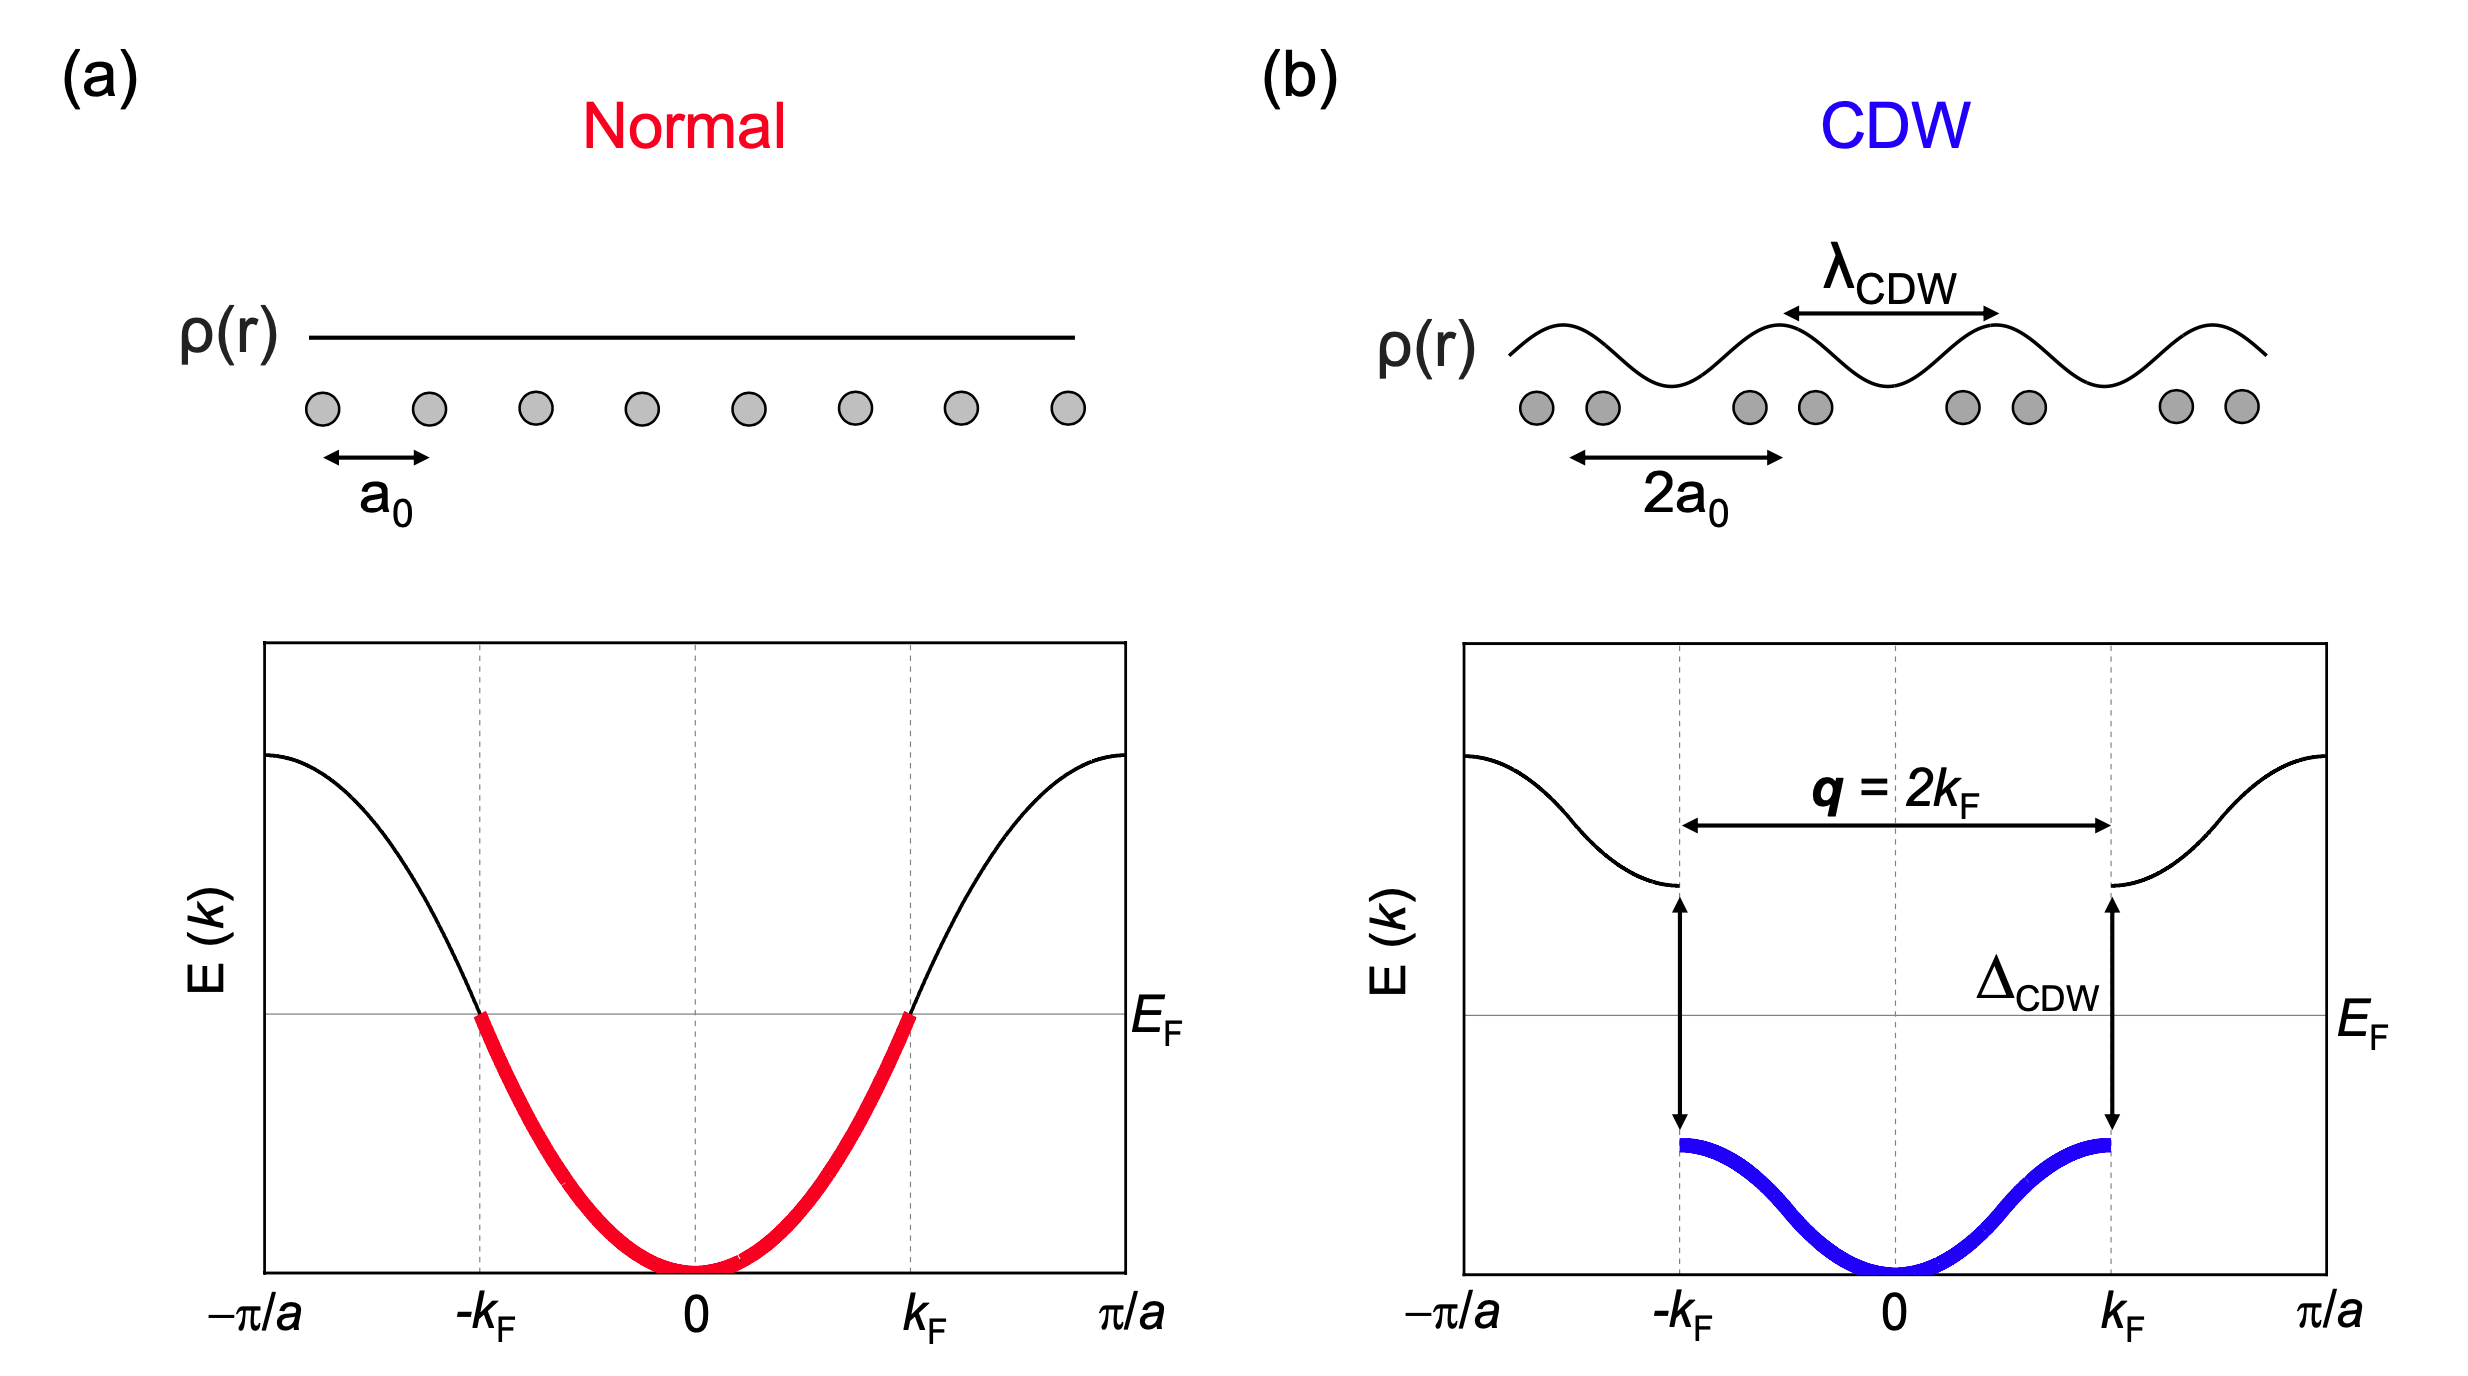
\includegraphics[width =\textwidth]{images/Peierls.png}
    \caption{Peierls transition is between (a)the normal state  and (b)the charge density wave state \cite{sayers2020charge}.  In the normal state, a one-dimensional chain with atom spacing $a_0$ has a uniform distribution of electron density and is half-filled at the ground state. In the charge density wave state, the lattice position becomes distorted, resulting in a modulation of the charge density wave. The unit cell becomes enlarged, and an energy band opens up a gap at the Fermi level.}
    \label{fig:Peierls}
\end{figure}

In this picture, the ground state of this system is the result of a competition between the electronic occupancy energy $E_{el}$ and the elastic energy of the lattice $E_{lat}$.
\begin{align}
    &E_{el} \sim -\frac{\Delta^2}{2}-\Delta^2\log(\frac{2E_F}{\Delta}) \\
    &E_{lat} \sim \frac{\Delta^2}{\lambda}
\end{align}
When the temperature is lowered, opening a gap reduces the energy of occupied electrons, but the distortion increases the elastic energy. The overall energy decreases, causing a metal-to-insulator phase transition in Peierls model.

CDWs are a state of matter characterized by a periodic modulation of the electron density in a material. This periodic modulation can be thought of as a "frozen" wave of electrons and ions. The CDW state is essentially a collective state of many electrons and ions. However, in real materials, impurities or defects are inevitable. These impurities or defects can "pin" the CDW, preventing it from moving freely through the material. This is known as the pinning of charge-density waves by impurities.

Pinning occurs because the impurities or defects disrupt the perfect periodicity of the CDW. When the CDW encounters an impurity, it can be deflected or scattered, causing it to lose coherence. This can prevent the CDW from moving or "sliding" through the material, effectively pinning it in place. The pinning of CDWs by impurities can have significant effects on the properties of the material. For example, it can lead to non-linear conduction properties, including threshold behavior (where the CDW does not move until the electric field exceeds a certain critical value) and non-Ohmic conduction (where the current is not proportional to the applied voltage).\cite{fukuyama1978dynamics,lee1979electric}

CDWs can be classified into two types: commensurate and incommensurate. A commensurate CDW is characterized by a charge density wavelength that is an integer multiple of the lattice constant. This alignment with the lattice allows the CDW to lower its energy, leading to a more stable state. However, this perfect alignment also makes the CDW more susceptible to pinning by impurities or defects within the lattice, which can disrupt the CDW's coherence. Conversely, an incommensurate CDW exhibits a periodicity that does not correspond to the underlying lattice's periodicity. This lack of alignment prevents the CDW from lowering its energy by aligning with the lattice, which can result in a less stable state. Interestingly, this misalignment can also be advantageous as it makes the CDW less susceptible to pinning by impurities or defects. The absence of perfect alignment allows the CDW to more effectively navigate around these disruptions, maintaining its wave-like properties.
\subsection{Origin of charge density wave}

One of the mechanism of CDW states is Fermi surface nesting(FSN). It means the shape of the Fermi surface enables match segment of the surface to be translated by a fixed vector in momentum space.  However, it is important to note that having two seemingly parallel pieces of the Fermi surface does not necessarily mean that it is nested. To determine the significance of nesting, the Lindhard susceptibility function must be calculated\cite{lindhard1954properties}. In one dimensional Peierls model, the Fermi surface is perfectly nested with vector $\mathbf{q}$ shown in fig\ref{fig:FSN}.

 \begin{figure}[h]
    \centering
    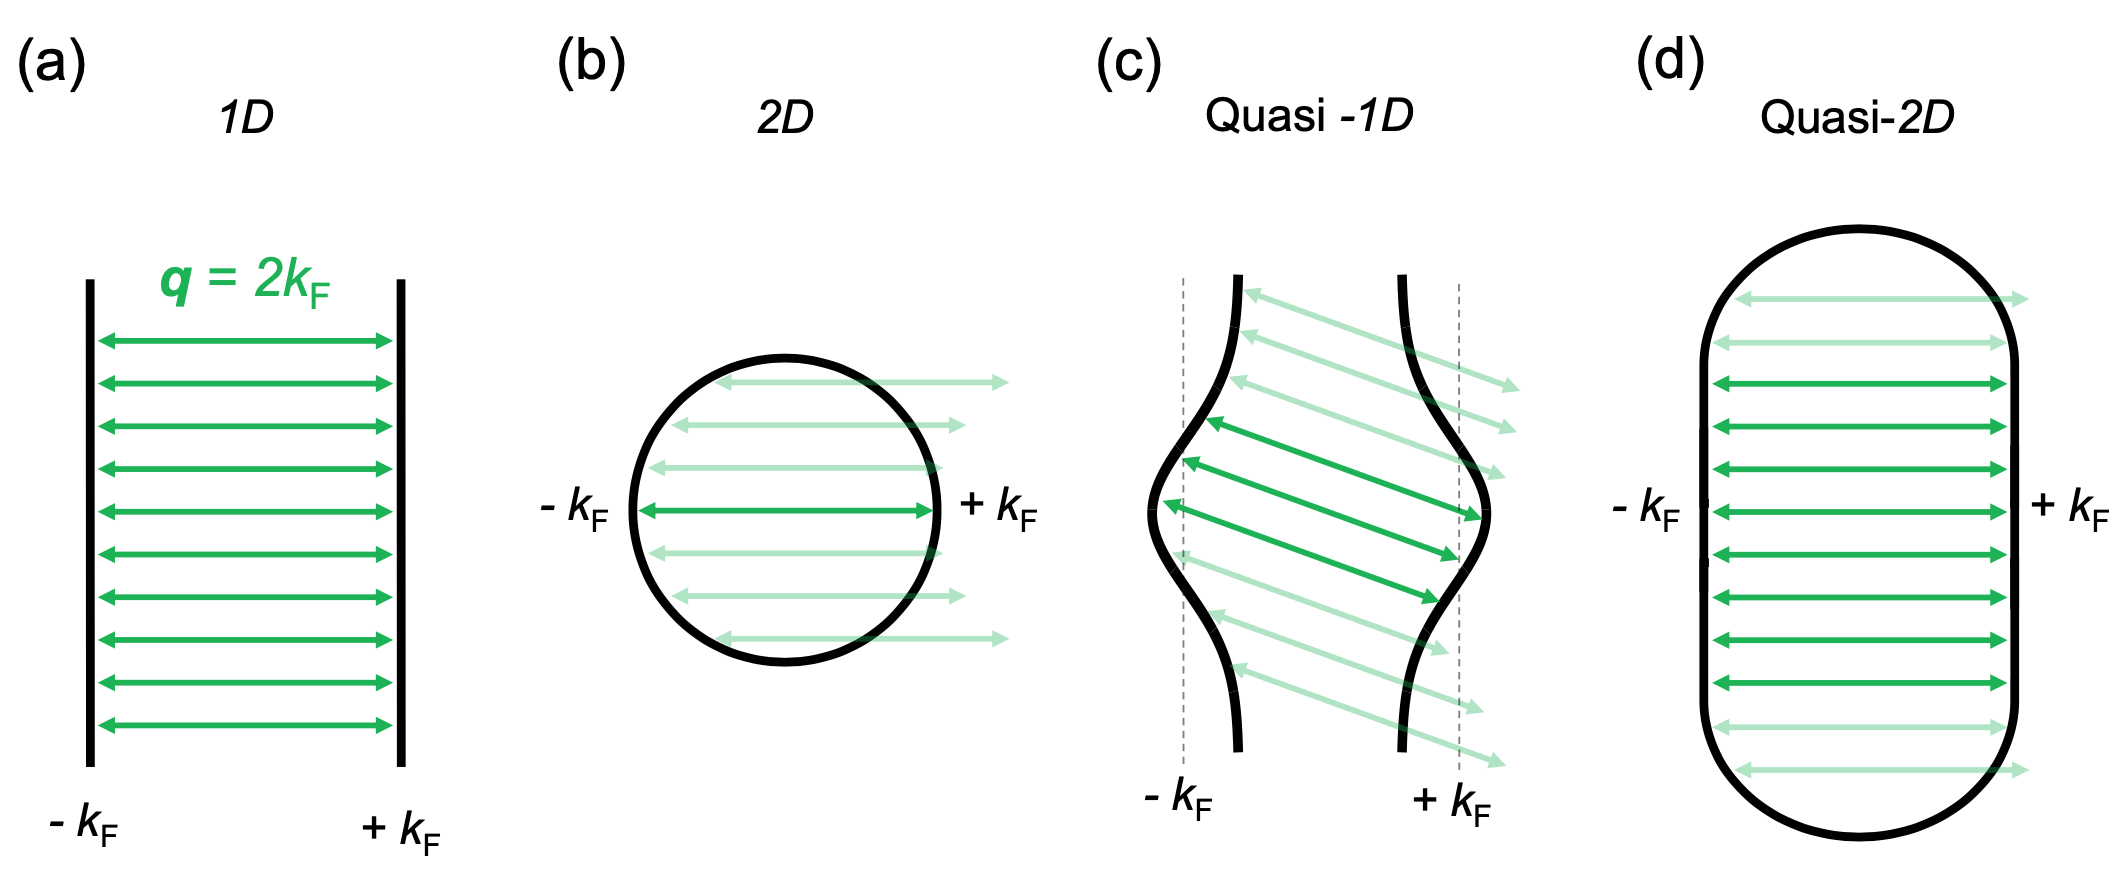
\includegraphics[width =\textwidth]{images/FSN.png}
    \caption{Fermi Surface Nesting(FSN) in different dimensions\cite{sayers2020charge}. (a) In one dimension, when the Fermi surface of a material has nearly parallel sections that can be connected by a single vector, called the nesting vector, the system can become unstable and undergo a Peierls transition to a CDW state. (b) Two dimensional cylindrical Fermi surface. There is no FSN. (c),(d) partial FSN are showing in quasi-1D and quasi-2D system. }
    \label{fig:FSN}
\end{figure}

As the dimensionality increases, the shape of the Fermi surface becomes more complex, and perfect nesting is rare.  There are lot of studies showed that the origin of CDW states doesn't falls into Peierls' picture. In a classic quasi-2D CDW material $NbSe_2$. The diffraction\cite{moncton1975study,du2000x} and STM\cite{arguello2014visualizing} measurements shows a CDW wave vector at $q_{CDW}\approx 0.7A^{-1}$ and CDW transition tempreture $T_{CDW}=33.5K$. However, resistivity measurements do not show evidence of a metal-insulator transition at $T_{CDW}$ and ARPES measurements\cite{zhu2015classification} shows no evidence of FSN. Thus, the origin of CDW in this system is not due to Fermi surface nesting but rather driven by electron-phonon coupling.

In summary, Fermi surface nesting is not the only mechanism responsible for the formation of CDWs\cite{johannes2008fermi}. The origin of CDWs can be attributed to the coupling between electronic and lattice degrees of freedom, as well as to the interplay between electronic interactions and the underlying crystal structure of the material.




\section{Higher order topological phases.}
\subsection{Bulk-boundary correspondence}
The existence of distinct topological classes of band structures has important practical implications, particularly in relation to the presence of anomalous boundary states. When the bulk band structure exhibits a nontrivial topology, it suggests the existence of these boundary states that cannot exist independently of the topological bulk. Anomalous boundary states are robust to local disturbances and can only be eliminated by perturbations that either close the excitation gap of the bulk band structure or reduce its symmetry. This relationship, known as bulk–boundary correspondence, establishes a direct link between the nontrivial topology of the bulk band structure and the presence of anomalous boundary states. In the case of topological phases governed solely by nonspatial symmetries, such as time-reversal symmetry or particle-hole antisymmetry in superconducting Bogoliubov–de Gennes Hamiltonians, the bulk–boundary correspondence is comprehensive. Like we have discussed in secontion \ref{sec:invariant}, it guarantees a unique association between each topological class of a $d$-dimensional bulk band structure and a corresponding anomalous boundary state in $d-1$ dimension.

The mathematical foundation of the bulk-boundary correspondence arises from the extension of the Atiyah-Singer (AS) index theorem to manifolds with boundaries\cite{fukui2012bulk, fukaya2020physicist, hatsugai1993chern, essin2011bulk}. The AS index theorem establishes an equivalence between the topological index associated with the bulk topology described by the Hamiltonian and the analytical index pertaining to the zero-energy states serving as solutions to the boundary differential equations. This can be summarized as follows:
\begin{align}
\text{Topological index} = \text{Analytical index}\\
\text{Bulk invariant} = \text{Boundary invariant}
\end{align}


The bulk–boundary correspondence becomes more intricate when considering topological phases that are protected by spatial symmetries like inversion or mirror symmetries. In such cases, the bulk–boundary correspondence is generally incomplete and necessitates a certain level of compatibility between the crystal termination and the crystalline symmetries. In 2011, Fu pioneered a three-dimensional model featuring topological phases protected by the combination of four-fold rotation symmetry and time reversal symmetry. This work paved the way for the exploration of topological crystalline insulators and superconductors \cite{fu2011topological}. The spectrum of crystalline symmetries capable of protecting topological phases spans from point group symmetry, such as inversion\cite{hughes2011inversion,lu2014inversion}, reflection\cite{hsieh2012topological, chiu2013classification}, and rotation symmetries, to space group symmetries like glide planes and screw axes\cite{po2017symmetry,slager2013space,kruthoff2017topological}. This exploration led to the introduction of novel topological invariants to characterize these phases.


After the discovery of topological crystalline insulators and superconductors\cite{ando2015topological, fu2011topological, hsieh2012topological, dziawa2012topological, liu2021bulk}, it became apparent that a conventional bulk–boundary correspondence, where the $(d-1)$-dimensional anomalous boundary states of a $d$-dimensional crystal , exists only for boundary orientations that preserves the same  crystalline symmetry as the bulk or remain unchanged under the action of the crystalline symmetry group. However, this condition is only valid for a restricted set of symmetry groups, such as mirror symmetry\cite{ando2015topological}, and even within those groups, it is limited to particular surface orientations.


\subsection{Extrinsic and intrinsic higher order topological phases}
So far, our discussion has focused on topological phases that exhibit boundary states in dimensions only one lower than the dimension of the bulk. More recently, in 2018 Schindler et al.\cite{schindler2018higher} and Khalaf\cite{khalaf2018higher} demonstrated that topological crystalline phases can exhibit anomalous boundary features of dimensions smaller than $(d-1)$-dimension, as long as the crystal termination as a whole respects the crystalline symmetry group. These anomalous states can manifest at hinges or corners of a 3D crystal or as  corner states in a 2D crystal. Notably, the criterion that the crystal termination as a whole respects to the crystalline symmetry group is a much weaker condition on the surface orientations compared to the requirement of individual crystal faces remaining invariant under the crystalline symmetry. Furthermore, this condition applies to all crystalline symmetry groups. Topological phases demonstrating this type of boundary feature are referred to as higher-order topological phases. A bulk topological phase of $n$-th order in $d$ dimensions manifests gapless states on a surface with a codimension of $d_c = n$. Under this classification scheme, conventional topological phases described in ten-fold table\ref{tab:10fold} are considered first-order $d_c=1$ in fig\ref{fig:HOTP}.  For instance, a three-dimensional first-order strong $\mathbb{Z}_2$ topological insulator features two-dimensional surface states (with $d_c = 1$). On the other hand, second-order and third-order topological insulators exhibit one-dimensional hinge modes with $d_c = 2$ and point-like corner states with $d_c = 3$, respectively.

 \begin{figure}[h]
    \centering
    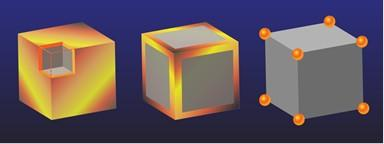
\includegraphics[width =0.8\textwidth]{images/TopologyFigure.jpg}
    \caption{The higher order topological phases with their boundary states with codimension $d_c = 1, 2,3$. A three-dimensional first-order strong topological material features two-dimensional surface states (with $d_c = 1$). Second-order and third-order topological phases exhibit one-dimensional hinge modes with $d_c = 2$ and point-like corner states with $d_c = 3$, respectively }
    \label{fig:HOTP}
\end{figure}

The higher order surface states not one depends on the bulk topology but also depends on the symmetry properties of system boundary. In this sense, the higher order topological phases(HOTPs) can be classified into two categories: extrinsic HOTPs and intrinsic HOTPs\cite{trifunovic2019higher, trifunovic2021higher,lei2022topological}. 


Extrinsic Higher-Order Topological Phases (HOTPs) are a characteristic of lattice terminations and do not depend on the bulk's topology. Nonetheless, they can still be protected by the $(d-1)$-dimensional boundary, which resides in a topological phase protected by local symmetries, while the $d$-dimensional bulk remains trivial. Extrinsic hinge states cannot be eliminated by perturbations that preserve crystalline symmetries and maintain the surface gap. Similarly, extrinsic corner states are robust against perturbations that preserve the symmetries and do not close the gaps on the hinges or surface. Their classification can be inherited from the topological classification of the $(d-1)$-dimensional boundary for symmetry protected topological  phases. Figure \ref{fig:Extrinsic} provides an example of extrinsic corner states, which emerge at the boundary of the topological upper edge. The topological corner states can be eliminated by introducing an additional nontrivial 1D chain to the same edge, as depicted in Figure \ref{fig:Extrinsic}(b), or they can be shifted to other corners by incorporating nontrivial 1D chains to the connected adjacent edges, as shown in Figure \ref{fig:Extrinsic}(c).

 \begin{figure}[h]
    \centering
    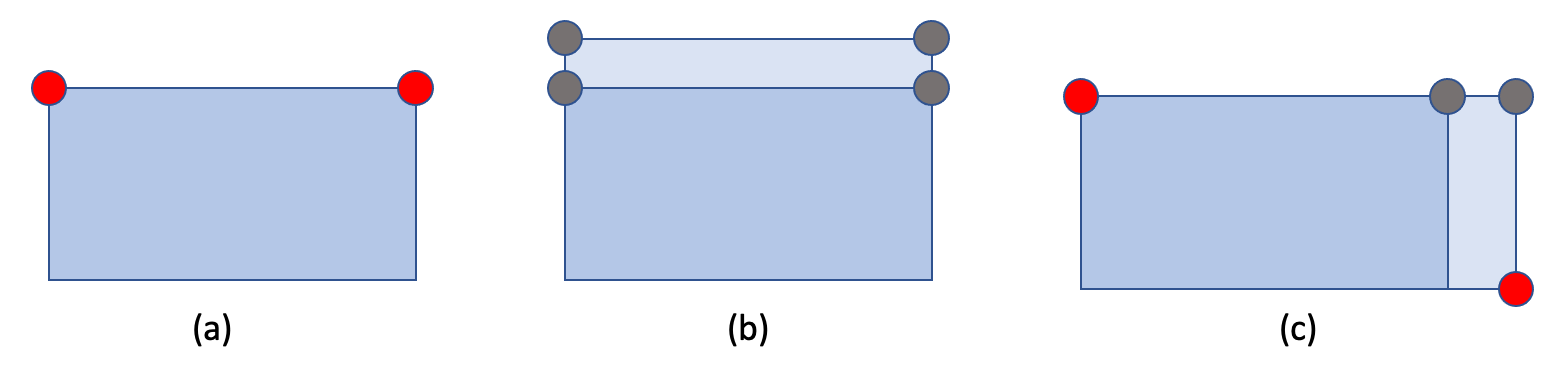
\includegraphics[width =\textwidth]{images/HOTI.png}
    \caption{ Extrinsic higher order topological corner states depends on the lattice termination.
(a) An illustration of extrinsic corner states, protected by the topologically non-trivial upper edge, is shown. These topological corner states can be gapped out by adding another nontrivial 1D chain to the same edge (b) or can be shifted to other corners by introducing nontrivial 1D chains to connected adjacent edges (c).}
    \label{fig:Extrinsic}
\end{figure}

Intrinsic HOTPs exhibit a distinct behavior compared to extrinsic HOTPs. Intrinsic HOTPs are characterized by topological states that cannot be displaced or removed by changing the system's termination if the termination maintains compatibility with a protecting crystalline symmetry. The higher order anomalous states are pinned to the corners or hinges as long as the gap in the bulk remains open. The requirement for the presence of topological states at the intersection of two boundaries is that these boundaries are related to each other by a crystalline symmetry operation. This condition is less stringent than that for topological crystalline phases, where crystal boundaries must remain invariant under the protecting crystalline symmetry to host topological states. \cite{trifunovic2019higher}

\subsection{HOTP in experiments}
\section{This theis}
In chapter2, we will talk about:

In chapter3, we will talk about:
...

% \lipsum[1-20]

\chapter{The Theory of PRex Experiment}
% \todo[inline]{Separate the theory and the experiment part into two chapters}

The RMS radius of the  neutron distribution in a heavy nucleus  $R_N$ provides an important test of nuclear theory. Furthermore   $R_N$ is used in the determination of  the density dependence of symmetry energy of neutron rich matter; this dependence is an  important input in   neutron star structure, heavy iron collision and atomic parity violation experiment calculations. In the past hadron scattering experiments with with pion, proton or anti-proton beams have been used to determine the neutron radii of heavy nuclei. However, these measurements suffer from uncertainties associated with the probe particle and the target nucleus. Electron scattering provides a model independent probe of nuclear radii.  However, in electron scattering, the measurement of neutron distribution in a nucleus  is much harder than the measurement of the proton distribution  since the neutron is uncharged. Because the  neutron weak charge is much large than that of the proton, PRex-II  used the parity violating weak neutral interaction to probe the neutron distribution in the  ${^{208}}Pb$ nucleus, thus measuring the RMS neutron radius with high  accuracy. The PRex-II experiment was performed from June to September 2019 in Jefferson lab experimental hall A using the High Resolution Spectrometer (HRS) pair. 

\section{electron scattering}

In 1961, Robert Hofstadter wins Nobel Price for his pioneering studies of structure of nucleons with  electron scattering. Accelerated electron beams are widely used for study the inner structure of the nucleons (and neutrons) since then. Those experiment can provide different level structure information of nucleons given different incident electron energy. At the range where the energy of electrons are very low, $\lambda \gg r_p$, here $r_p$ is the radius of the proton, $\lambda$ is the electron wavelength, the scattering is equivalent to scattered over point like spin-less object. At low electron energy range where $\lambda ~r_p$, the scattering is equivalent to scattering over charged object. When the electron wavelength $\lambda < r_p$, the electron scattering will be able to see the substructures. At very high energy range where $\lambda \ll r_p$, the electrons is equivalent to scattering over the sea of quarks and gluons of the protons. 

In one photon exchange approximation, the transition current of electron can be write as:
$$
j^\mu = - e\bar{\mu}_e(k')\gamma^\mu\mu_e(k)e^{i\vec{q}\vec{x}}
$$

The  transition current for nucleon can be write as:

$$
J^\mu = e\bar{\mu}\Gamma^\mu(p)e^{i\vec{q}\vec{x}}$$
$$

\todo[inline]{Add the Feynman diagram}

In one photon exchange approximation, the cross section of electron scattered over spin-0 particle would be:

$$
\frac{d\sigma}{d\Omega} = \frac{d\sigma}{d\Omega}|_{mott}*|F(Q^2)|^2
$$

\todo[inline]{current result of proton radius (PRad)}

\subsection{e-p scattering}
\subsection{e-n scattering}
\subsection{form factor}

\section{Weak interaction and weak current}
\section{Parity Violation}
\section{Parity Violation Asymmetry}
\todo[inline]{derive the asymmetry in term of form factor}
\section{Rich Physics Behind the PRex Experiment}
\subsection{EOS of Neutron rich matter}
  \chapter{The High Resolution Spectrometer Optimization(30)}

Introduction:
\begin{itemize}
    \item apparatus
    \item why we need to Optics 
    \item how to do optics (linear regression))
    \item a brief of the result
\end{itemize}


% \lipsum[1-20]
\section{Apparatus}

\begin{itemize}
    \item Overview of the HRS structure
    \item septum magnet 
    \item Vertical drift chamber 
    \item GEM detector
    \item supporting equipment used for optimization only sieve slide

    \item coordination system of the Jefferson Lab Hall A
    \item coordination system of the HRS
\end{itemize}


\section{HRS model}

\begin{itemize}
    \item math why higher order contribute, a discussion notes
    \item feature selection technics
    \item linear regression
    \item result validation
    \item result and discussion
\end{itemize}

\subsection{Linear Regression and mathematics approximation}






\section{feature selection}

\subsection{general consideration in regression}

\subsection{features in regression}

\subsection{LASSO feature reduction regression}

\subsection{ridge feature reduction regression}

\subsection{autoML and more}

\section{Momentum optimization}

\section{Regression Result validation}

\subsection{carbon result check}

\subsubsection{first, second, third momentum check}

\section{momentum reconstruction}

\section{scattered angle reconstruction and correction}

\section{a second thought/attempt on the regression}

\subsection{another more complicated model}
\chapter{Theoretical Overview}

\lipsum[1-20]

\chapter{Results}

\lipsum[1-20]

\chapter{Summary and Conclusion}

% \lipsum[1-20]

\appendix
% -*-latex-*-

\chapter{Appendix A}

\clearpage
\newpage

%%%%%%%%%%%%%%%%%%%%%%%%%%%%%%%%%%%%%%%%%%%%%%%%%%%%%%%%%%%%%%%%%%%%%%
% -*-latex-*-


\cleardoublepage
\pdfbookmark[0]{Bibliography}{Bibliography}
% -*-latex-*-

%% This defines the bibliography file (main.bib) and the bibliography style.
%% If you want to create a bibliography file by hand, change the contents of
%% this file to a `thebibliography' environment. For more information, see
%% section 4.3 of the LaTeX manual.

\begin{singlespace}
\bibliography{main}
\bibliographystyle{plain}
\end{singlespace}

%%%%%%%%%%%%%%%%%%%%%%%%%%%%%%%%%%%%%%%%%%%%%%%%%%%%%%%%%%%%%%%%%%%%%%
% -*-latex-*-

\cleardoublepage

\end{document}
